% Definerer format på dokumentet
\documentclass[12pt]{scrbook}

% Importerer pakker og ordner formatering
\usepackage{setup}

% Setter linjeavstand
\linespread{1.5} 

% Dokument start
\begin{document}

\pagenumbering{roman}   % Setting page numbering to lower-case roman

% Forord og sammendrag
\chapter*{Forord}

% Skriv forord her

Forordet skal avsluttes med følgende tekst:
Innholdet i denne oppgaven står for forfatternes regning.

Dersom dere skal skrive på engelsk kan tittel endres til 'Preface' og dere må avslutte forordet med føldende tekst:
The authors take full responsibility for the content of this thesis.

\vfill
\noindent Trondheim, 2024
\vspace{0.5cm}


\begin{table}[H]
    \centering
    \begin{tabular}{ccccc}
    \multicolumn{2}{c}{
\includegraphics[width = 11em]{images/signatur.png}} & \quad\quad\quad\quad\quad & \multicolumn{2}{c}{
\includegraphics[width = 11em]{images/signatur.png}}\\
    \multicolumn{2}{c}{Navn Navnesen} &  & \multicolumn{2}{c}{Navn Navnesen}\\
    \end{tabular}
\end{table}
\chapter*{Sammendrag}
Skriv sammendrag på norsk her.
\chapter*{Abstract}
Skriv sammendrag på engelsk her.

% Innholdsfortegnelse
\tableofcontents

% Liste over figurer og tabeller
\listoffigures
\listoftables

% Forkortelser
\chapter*{Forkortelser}

\begin{tabular}{>{\bfseries}rl}
       LR & Logistisk regresjon \\
       NR  & Nøyaktighetsratio  \\
\end{tabular}

\pagenumbering{arabic}  % Setting page numbering to normal integers

% Legger inn oppgavens kapitler her
\chapter{Introduksjon}\label{chap:Introduksjon}

This template uses the Norwegian format. To switch to English, modify the language at the top of the 'setup.sty' file.

Denne malen oppdateres av Ranik Raaen Wahlstrøm. Vennligst si ifra hvis du oppdager feil ved malen eller hvis du har forslag til forbedringer.

Denne malen garanterer ikke at den oppfyller eventuelle formkrav gitt av ditt institutt. Sørg derfor for å tilpasse den slik at alle formkrav som gjelder for deg blir oppfylt.

Oppdatert utgave av malen finnes til enhver tid på denne linken:\\
\href{https://masterthesistemplate.ranik.no}{https://masterthesistemplate.ranik.no}

Flere LaTeX maler fra NTNU kan finnes her:\\
\href{https://www.overleaf.com/edu/ntnu#templates}{https://www.overleaf.com/edu/ntnu\#templates}

%Delkapittel
\section{Henvisninger}
% Lager label som kan referere til delkapittelet i teksten
\label{sec:Henvisninger}

Eksempler på hvordan dere kan henvise til kapitler, seksjoner, appendiks, tabeller og figurer i teksten:

kapittel \ref{chap:data}

seksjon \ref{sec:Henvisninger}

appendiks \ref{appendix:variabler}

tabell \ref{tab:simulation_1:industry}

figur \ref{fig:simulation_proportions}

ligning (\ref{eq:AR})


\subsection{Henvisning til kilder}
Bruk cite\{\} og citep\{\} for å referere i teksten. Eksempler:

\citep{paraschiv_bankruptcy_2021} 

\cite{paraschiv_bankruptcy_2021}

For å oppgi tekst før og etter kilden i samme parenteser: \citep[for eksempel][side 3]{paraschiv_bankruptcy_2021}

Flere kilder i samme parenteser: \citep{paraschiv_bankruptcy_2021,kamal_cryptocurrencies_2023} 





\section{Forskningsspørsmål}\label{sec:forskningsspm}
Vi har dermed følgende problemstilling:

% Midtstiller og legger teksten i kursiv
\begin{center}
\textit{Hva er problemstillingen?}
\end{center}


\section{Oppgavens struktur}
\chapter{Litteraturgjennomgang og teoretisk bakgrunn}




\chapter{Data og variabler}\label{chap:data}

\chapter{Metode}

Her er eksempler på hvordan ligninger kan skrives. Husk å definere alle symboler som brukes i ligningene.

\section{Eksempel fra \cite{kamal_cryptocurrencies_2023}}

For each cryptocurrency $i$, we calculate abnormal return (AR) by 
\begin{equation}\label{eq:AR}
    AR_{i,t} = R_{i,t} - E\left(R_{i,t}\right)
\end{equation}
where $R_{i,t}$ is the hourly log return, and $E\left(R_{i,t}\right)$ is the expected return calculated as the average of $R_{i,t}$ over a 30 days estimation window ending 36 hours before the event hours for the threat and act events. Further, we calculate the cumulative abnormal return (CAR) over the event window $\left[ \tau_1,\tau_2 \right]$ by
\begin{equation}
    CAR_i\left[ \tau_1,\tau_2 \right] = \sum_{t=\tau_1}^{\tau_2} AR_{i,t} 
\end{equation}

\section{Eksempel fra \cite{paraschiv_bankruptcy_2021}}


When using LR as estimation technique, the vector of predicted probabilities for bankruptcy $\mathbf{\hat{y}}=\{\hat{y}_n\}_{n=1,\dots,N} \in [0,1]^N$ 
is given by
\begin{equation}\label{LR:predicted probability}
\mathbf{\hat{y}} = \mathbf{\iota} \oslash \left( \mathbf{\iota} +\exp\left(- \mathbf{X} \mathbf{w} - \mathbf{\iota} w_0 \right) \right)
\end{equation}
where $\mathbf{X}=\{x_{(n,i)}\}_{n=1,\dots,N,i=1,\dots,I}$ is a matrix of values for input variables $i$ derived from the financial statements $n$, $\mathbf{w}=\{w_i\}_{i=1,\dots,I}$ is a vector of coefficients, $w_0$ is the intercept coefficient, $\mathbf{\iota}$ is an $N \times 1$ vector of ones, and $\oslash$ denotes Hadamard (element-wise) division. For ease of notation, we drop the time indices. 
\chapter{Resultater og diskusjon}

Her følger noen eksempler på tabeller og figurer. Alle er hentet fra \cite{paraschiv_bankruptcy_2021}.

\begin{table}[h]
  \centering
\captionof{table}{\textbf{Simulation of a competitive credit market with two banks -- general versus industry-specific datasets}}\label{tab:simulation_1:industry}
    \begin{tabular}{l|rr}
    \hline\hline
          & \textbf{LAS} & \textbf{LIN}  \\
          \hline
    \textbf{Market share of each bank in EUR (\%)} &  50.8  &  49.1   \\
    \textbf{Share of bankrupting borrowers in portfolio (\%)} &  2.7  & 1.9  \\
    \textbf{Share of bankrupting borrowers in the market (\%)} & 57.1  &    34.6  \\
    \textbf{Revenue} &    55,854.8  &    50,954.0 \\
    \textbf{Loss} &    24,169.3  &    17,302.1   \\
    \textbf{Profit} &    31,685.5  &    33,652.0   \\
    \textbf{Profit margin (\%)} & 56.7  & 66     \\
    \textbf{Return on assets (ROA) (\%)} & 0.3   & 0.4    \\
    \textbf{Return on risk-weighted assets (RORWA) (\%)} & 0.5   & 0.6   \\
    \hline\hline
    \end{tabular}
    % \bigskip
  \caption*{Tabelltekst her. Teksten bør være så utfyllende at leseren skjønner hva tabellen forteller uten å måtte se i hovedteksten.}
\end{table}



\begin{figure}[h]
\captionof{figure}{\textbf{Stability of variable selection}}\label{fig:number of unique input variables}
	\centering
	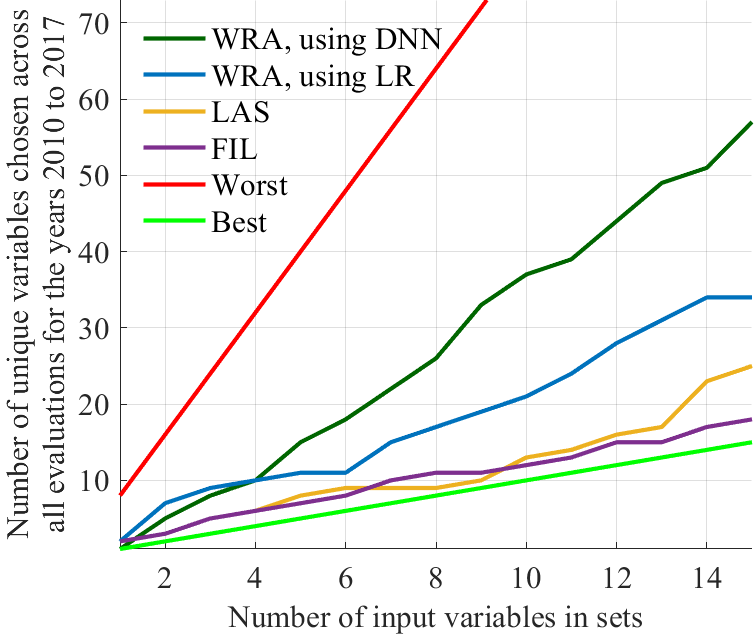
\includegraphics[width=0.49\linewidth]{images/unique_input_variables.png}
	% \bigskip
 	\caption*{Figurtekst her. Teksten bør være så utfyllende at leseren skjønner hva figuren forteller uten å måtte se i hovedteksten.}
\end{figure}


\begin{figure}[h]
  	\begin{center}
  	\captionof{figure}{\textbf{Total cumulative amount lent within percentiles of amount borrowers are willing to borrow -- General versus industry-specific variable sets}}
  	\label{fig:simulation_proportions}
  	\captionsetup{justification=centering}
  	 \begin{subfigure}[t]{0.47\linewidth}
  	 \vspace{0.4cm}
  	        \caption*{\large Panel A}
  	        \vspace{-0.3cm}
    		\includegraphics[width=\linewidth]{"images/pst_cum_captured_non_bankrupt".png}
  	\end{subfigure}
 	\begin{subfigure}[t]{0.47\linewidth}
 	\vspace{0.4cm}
            \caption*{\large Panel B}
            \vspace{-0.3cm}
    		\includegraphics[width=\linewidth]{"images/pst_cum_captured_bankrupt".png}
  	\end{subfigure}
  	\vspace{-0.6cm}
  	\end{center}
  \caption*{Tabelltekst her. Teksten bør være så utfyllende at leseren skjønner hva tabellen forteller uten å måtte se i hovedteksten.}
\end{figure}
\chapter{Konklusjon}


%%%%%%%%%%%%%%%%%%%
%% Referanselisten
%%%%%%%%%%%%%%%%%%%
\clearpage
\addcontentsline{toc}{chapter}{Referanser} % Gjør så referansene havner i innholdsfortegnelsen
\renewcommand{\bibname}{Referanser} % Her defineres overskriften
\linespread{1.0}  % Singlespacing for å ha litt mindre linjeavstand i referanselista
\bibliographystyle{elsarticle-harv-nourl} % Definerer stilen, denne hentes fra en egen fil. Dette er Harvard stil
\bibliography{references} % Dette er navnet på .bib-filen hvor dere har lagret referansene (bruk gjerne et kildehåndteringsprogram, slik som Zotero)
\linespread{1.5} % Setter linjeavstand tilbake til den som benyttes i oppgaven ellers



%%%%%%%%%%%%%%%%%%%%%%%%%%%%%%%%%%%%%%
%% Appendices
%%%%%%%%%%%%%%%%%%%%%%%%%%%%%%%%%%%%%
\appendix
% \renewcommand{\thechapter}{Appendix \Alph{chapter}}

% Gjør så alle figurer og tabeller i appendikset har A. foran seg
\setcounter{table}{0}
\setcounter{figure}{0}
\renewcommand\thetable{A.\arabic{table}} 
\renewcommand\thefigure{A.\arabic{figure}} 

\chapter{Variabler} \label{appendix:variabler}

I dette appendikset gis det eksempel på en tabell som strekker seg over flere sider. Tabellen er hentet fra \cite{paraschiv_bankruptcy_2021}.

\captionof{table}{\textbf{Input variables for bankruptcy prediction}}\label{tab:Input variables considered in this study}
\caption*{Tabelltekst her. Teksten bør være så utfyllende at leseren skjønner hva tabellen forteller uten å måtte se i hovedteksten.}
\singlespacing
\begin{longtable}{l|r}
\textbf{Description}&\textbf{PCC}\\
\hline
\endfirsthead
\caption*{\textbf{Tabell \ref{tab:Input variables considered in this study}:} Input variables for bankruptcy prediction (continued)}\\
\addtocounter{table}{-1} 
\textbf{Description}&\textbf{PCC}\\
\hline
\endhead
\endfoot
\hline
    accounts payable / total assets & 0.17  \\
    dummy; one if total liability exceeds total assets & 0.16  \\
    total equity / total assets & - 0.15  \\
    (current liabilities - short-term liquidity) / total assets & 0.15  \\
    total liabilities / total assets & 0.15  \\
    current liabilities / total assets & 0.15  \\
    net income / total assets & - 0.13  \\
    retained earnings / total assets & - 0.13  \\
    dummy; one if paid-in equity is less than total equity & - 0.13  \\
    pre-tax profit / total assets & - 0.13  \\
    EBIT / total assets & - 0.12  \\
    working capital / total assets & - 0.12  \\
    EBIT / total tangible assets & - 0.12  \\
    operating profit / total assets & - 0.12  \\
    EBITDA / total assets & - 0.11  \\
    (short-term assets - total liabilities) / total assets & - 0.11  \\
    interest expenses / total assets & 0.11  \\
    public taxes payable / total assets & 0.10  \\
    total expenses / assets & 0.10  \\
    operating expenses / total assets & 0.10  \\
    (non-interest expenses - salary) / total assets & 0.09  \\
    accounts payable / current liabilities & 0.09  \\
    sales / total tangible assets & 0.08  \\
    sales / current assets & 0.08  \\
    sales / total assets & 0.08  \\
    (shareholder’s equity + total revenues) / total assets & 0.08  \\
    total revenues / total assets & 0.08  \\
    investment turnover (sales / (total equity + total liabilities)) & 0.08  \\
    net income / (total liabilities + paid-in capital) & - 0.07  \\
    inventory / current assets & 0.07  \\
    retained earnings / tangible assets & - 0.07  \\
    operating profit / paid-in capital & - 0.07  \\
    log(age in years) & - 0.07  \\
    short-term liquidity / current assets & - 0.07  \\
    salary / total assets & 0.06  \\
    (current assets - short-term liquidity) / total assets & 0.06  \\
    pre-tax profit / paid-in capital & - 0.06  \\
    net income / paid-in capital & - 0.06  \\
    short-term liquidity / total assets & - 0.05  \\
    log(total assets) & - 0.05  \\
    effective tax rate & - 0.05  \\
    retained earnings / inventory & - 0.05  \\
    working capital / long-term liabilities & - 0.05  \\
    total equity / long-term liabilities & - 0.04  \\
    interest income / total assets & - 0.04  \\
    dividends / net income & - 0.03  \\
    quick assets / sales & - 0.03  \\
    sales / tangible assets & 0.03  \\
    net quick assets / inventory & - 0.03  \\
    operating expenses / sales & - 0.03  \\
    (total revenues - sales) / total revenues & - 0.03  \\
    short-term liquidity / sales & - 0.03  \\
    total equity / (total equity + long-term liabilities) & - 0.03  \\
    operating profit / total revenues & 0.03  \\
    total equity / fixed assets & - 0.03  \\
    short-term liquidity as a percentage of the capital employed & - 0.03  \\
    quick assets /total assets & - 0.03  \\
    interest income / interest expenses & - 0.03  \\
    long-term liabilities / total assets & 0.03  \\
    sales / short-term liquidity & 0.02  \\
    EBIT / interest expense & - 0.02  \\
    current liabilities / total equity & - 0.02  \\
    sales / total equity & - 0.02  \\
    intangibles / total assets & 0.02  \\
    current assets / total equity & - 0.02  \\
    (total revenues + interest income) / total expenses & - 0.02  \\
    sales / working capital & - 0.02  \\
    total liabilities / total equity & - 0.02  \\
    total revenues / net working capital & - 0.02  \\
    working capital / operational expenditure & - 0.02  \\
    total revenues / sales & - 0.02  \\
    current assets / total assets (net liquid assets / total assets) & 0.02  \\
    fixed assets / total assets & - 0.02  \\
    fixed assets / total equity & - 0.02  \\
    (long-term liabilities + total equity) / fixed assets & - 0.02  \\
\end{longtable}

\linespread{1.5} % Setter linjeavstand tilbake til den som benyttes i oppgaven ellers

\chapter{Resultater av robusthetstester} \label{appendix:Resultater av robusthetstester}




% Dokument slutt
\end{document}
